
%!TEX encoding = UTF-8 Unicode
%!TEX root = ../exercises.tex

\ifPreSolution



\Exercise{\ExeWeekSIX}\label{exe:W06}

\begin{Goals}
%!TEX encoding = UTF-8 Unicode
%!TEX root = ../compendium2.tex

\item Kunna läsa och skriva pseudokod för sekvensalgoritmer och implementera sekvensalgoritmer enligt pseudokod.

\item Kunna implementera sekvensalgoritmer, både genom kopiering till ny sekvens och genom förändring på plats i befintlig sekvens.

\item Kunna använda inbyggda metoder för uppdatering av, linjärsökning i, och sortering av sekvenssamlingar.

\item Kunna beskriva skillnaden i användningen av föränderliga och oföränderliga sekvenser, speciellt vid uppdatering.

\item Kunna implementera linjärsökning enligt olika sökkriterier.

\item Kunna beskriva egenskaperna hos sekvenssamlingarna \code{Vector}, \code{List}, \code{Array}, \code{ArrayBuffer} och \code{ListBuffer}.

\item Förstå bieffekter av uppdatering av delade referenser till föränderliga element.

\item Kunna använda funktioner med repeterade parametrar.

\item Känna till hur man implementerar funktioner med repeterade parametrar.

\item Kunna implementera heltalsregistrering i en heltalsarray.

\item Kunna beskriva skillnader i syntax mellan arrayer i Scala och Java.

\item Kunna beskriva skillnader i syntax och semantik mellan enkla for-satser i Scala och Java.


\item Känna till hur klassen \code{java.util.Scanner} kan användas för att skapa heltalssekvenser ur strängsekvenser.

\end{Goals}

\begin{Preparations}
\item \StudyTheory{06}
\end{Preparations}

\BasicTasks %%%%%%%%%%%%%%%%

\else



\ExerciseSolution{\ExeWeekSIX}


\BasicTasks %%%%%%%%%%%

\fi





\WHAT{Variabelt antal argument.}

\QUESTBEGIN

\Task  \what~  Det går fint att deklarera en funktion som tar en argumentsekvens av godtycklig längd. Syntaxen består av en asterisk \code{*} efter typen.

\Subtask Vad händer nedan?
\begin{REPL}
scala> def printAll(xs: Int*) = xs.foreach(println)
scala> printAll(42)
scala> printAll(1, 2, 7, 42)
scala> def printStrings(wa: String*) = println(wa)
scala> printStrings("hej","på","dej")
\end{REPL}

\Subtask Vad har parametern \code{wa} i \code{printStrings} ovan för typ?

\Subtask Ändra i \code{printAll} så att även längden på \code{xs} skrivs ut före utskriften av alla element. Testa att anropa \code{printAll} med olika antal parametrar.

\Subtask Vad händer om du anropar \code{printAll} med noll parametrar?

\SOLUTION


\TaskSolved \what
 

\SubtaskSolved  42;\\
 1\\
 2\\
 7\\
 42;\\
 WrappedArray(hej, på, dej)

\SubtaskSolved  WrappedArray

\SubtaskSolved  def printAll(xs: Int*) = {println(xs.size); xs.foreach(println)}

\SubtaskSolved  Storleken “0” skrivs ut och inget annat.




\QUESTEND




%%<AUTOEXTRACTED by mergesolu>%%      % Uppgift 1




\WHAT{Oföränderliga sekvenser med föränderliga objekt.}

\QUESTBEGIN

\Task  \what~ 

\Subtask Vad får xs för värde efter att attributet i objektet som \code{c2} refererar till ändras på rad 4 nedan? Förklara vad som händer.
\begin{REPL}
scala> class IntCell(var x: Int){override def toString = "[Int](" + x + ")"}
scala> val (c1, c2, c3) = (new IntCell(7), new IntCell(8), new IntCell(9))
scala> val xs = Vector(c1, c2, c3)
scala> c2.x = 42
scala> xs
\end{REPL}

\Subtask\Pen Rita en bild av minnessituationen efter rad 4 ovan.

\Subtask\Pen Vad krävs för att allt innehåll i en oföränderlig samling garanterat ska förbli oförändrat?

\SOLUTION


\TaskSolved \what
 

\SubtaskSolved  \begin{REPL}
scala.collection.immutable.Vector[IntCell] =
    Vector([Int](7), [Int](42), [Int](9))
\end{REPL}
Referensena till c2 och xs ändras aldrig.
xs kommer fortfarande ha tre vektorer som refererar till c1, c2, c3, däremot refererar dessa i sin tur till var sin int som är Mutable.
I detta fallet ändras c2.x:s referens från 8 till 42.

\SubtaskSolved  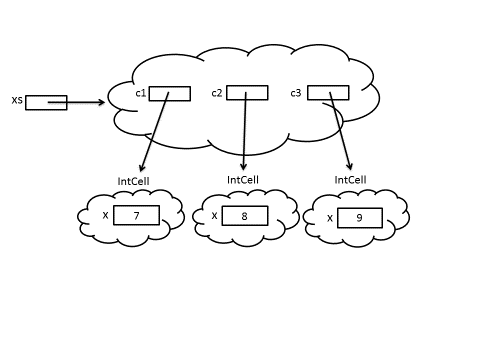
\includegraphics{../img/w05-solutions/memory-pic-1}

\SubtaskSolved  Istället för att skriva \code{IntCell(var x: Int)} så kan man skriva \code{IntCell(val x: Int)} där varje cells intvärde kommer vara oförändlig.
Alltså då attributen till objekten är “Val” så kommer även de att vara oförändliga.



\QUESTEND




%%<AUTOEXTRACTED by mergesolu>%%      % Uppgift 2




\WHAT{NEEDS A TOPIC DESCRIPTION}

\QUESTBEGIN

\Task  \what~ Föränderliga, indexerbara sekvenser: \code{Array} och \code{ArrayBuffer}

\Subtask Samlingen \code{scala.Array} har speciellt stöd i JVM och är extra snabb att allokera och indexera i. Dock kan man inte ändra storleken efter att en Array allokerats. Behöver man mer plats kan man kopiera den till en ny, större array. Koden nedan visar hur det kan gå till.
\begin{REPL}
scala> val xs = Array(42, 43, 44)
scala> val ys = new Array[Int](4)  //plats för 4 heltal, från början nollor
scala> for (i <- 0 until xs.size){ys(i) = xs(i)}
scala> ys(3) = 45
\end{REPL}
Definiera funktionen \code{def copyAppend(xs: Array[Int], x: Int): Array[Int]} som implementerar nedan algoritm, \emph{efter} att du rätta de \textbf{\color{red}{två buggarna}} i algoritmens while-loop:

\begin{algorithm}[H]
 \SetKwInOut{Input}{Indata}\SetKwInOut{Output}{Resultat}

 \Input{Heltalsarray $xs$ och heltalet $x$}
 \Output{En ny array som som är en kopia av $xs$ men med $x$ tillagt på slutet som extra element.}
 $n \leftarrow$ antalet element i $xs$ \\
 $ys \leftarrow$ en ny array med plats för $n + 1$ element\\
 $i \leftarrow 0$  \\
 \While{$i \leq n$}{
  $ys(i) \leftarrow xs(i)$
 }
 $ys(n) \leftarrow x$
\end{algorithm}



\Subtask Samlingen \code{scala.collection.mutable.ArrayBuffer} är inte riktigt lika snabb i alla lägen som \code{scala.Array} men storleksändring hanteras automatiskt, vilket är en stor fördel då man slipper att själv implementera algoritmer liknande \code{copyAppend} ovan. Speciellt använder man ofta \code{ArrayBuffer} om man stegvis vill bygga upp en sekvens. Vad händer nedan?
\begin{REPL}
scala> val xs = scala.collection.mutable.ArrayBuffer.empty[Int]
scala> xs.append(1, 1)
scala> while (xs.last < 100) {xs.append(xs.takeRight(2).sum); println(xs)}
scala> xs.last
scala> xs.length
\end{REPL}

\Subtask Talen i sekvensen som produceras ovan kallas Fibonaccital\footnote{\href{https://sv.wikipedia.org/wiki/Fibonaccital}{sv.wikipedia.org/wiki/Fibonaccital}}. Hur lång ska en Fibonacci-sekvens vara för att det sista elementet ska komma så nära (men inte över) \code{Int.MaxValue} som möjligt?



\SOLUTION


\TaskSolved \what
 

\SubtaskSolved  \begin{Code}
def copyAppend(xs: Array[Int], x: Int): Array[Int] = {
  val n = xs.size
  val ys = new Array[Int](n+1)
  var i = 0
  while(i < n) {
    ys(i) = xs(i)
    i += 1
  }
  ys(n) = x
  ys
}
\end{Code}

\SubtaskSolved  \begin{REPL}
xs: scala.collection.mutable.ArrayBuffer[Int] = ArrayBuffer()
ArrayBuffer(1, 1, 2)
ArrayBuffer(1, 1, 2, 3)
ArrayBuffer(1, 1, 2, 3, 5)
ArrayBuffer(1, 1, 2, 3, 5, 8)
ArrayBuffer(1, 1, 2, 3, 5, 8, 13)
ArrayBuffer(1, 1, 2, 3, 5, 8, 13, 21)
ArrayBuffer(1, 1, 2, 3, 5, 8, 13, 21, 34)
ArrayBuffer(1, 1, 2, 3, 5, 8, 13, 21, 34, 55)
ArrayBuffer(1, 1, 2, 3, 5, 8, 13, 21, 34, 55, 89)
ArrayBuffer(1, 1, 2, 3, 5, 8, 13, 21, 34, 55, 89, 144)
Int = 144
Int = 12
\end{REPL}

\SubtaskSolved  \code{xs.size = 46}\\
\code{xs(45) = 1836311903}\\
(Ha en arrayBuffer av typen Long istället och byt 100 mot Int.MaxValue och ta det nästsista elementet i sekvensens (det sista kommer vara över))


\QUESTEND




%%<AUTOEXTRACTED by mergesolu>%%      % Uppgift 3




\WHAT{Kopiering och uppdatering.}

\QUESTBEGIN

\Task  \what~  Metoder på oföränderliga samlingar skapar nya samlingar istället för att ändra. Därför behöver man inte själv skapa kopior. När en \emph{föränderlig} samling uppdateras på plats, syns denna förändring via alla referenser till samlingen.

\begin{REPL}
scala> val xs = Vector(1, 2, 3)
scala> val ys = xs.toArray
scala> ys(1) = 42
scala> xs
scala> ys
scala> val zs = ys.toArray
scala> zs(1) = 84
scala> xs
scala> ys
scala> zs
\end{REPL}

\Subtask Syns uppdateringen av objektet som \code{ys} refererar till via referensen \code{xs}? Varför?

\Subtask Syns uppdateringen av objektet som \code{zs} refererar till via referensen \code{ys}? Varför?

\Subtask Syns uppdateringen av objektet som \code{zs} refererar till via referensen \code{xs}? Varför?

\SOLUTION


\TaskSolved \what
 

\SubtaskSolved  Nej det gör det inte.
Då ys tilldelas xs.toArray kopieras datan från xs över i en array (som är mutable) vilket är en annan referens än den till xs.
Detta innebär att xs och ys inte “pekar” på samma objekt längre.

\SubtaskSolved  Ja därför båda är array och nu kopieras referensen till ys över till zs.
Därför kommer alla ändringar i zs att påverka ys (så länge de pekar på samma referens).

\SubtaskSolved  Nej det gör det inte. Se a).



\QUESTEND




%%<AUTOEXTRACTED by mergesolu>%%      % Uppgift 4




\WHAT{Färdig metod för att skapa kopia av array.}

\QUESTBEGIN

\Task  \what~  Om man inte vill att en uppdatering av en föränderlig samling ska få oönskad påverkan på andra koddelar som refererar till samlingen, behöver man göra kopior av samlingen före uppdatering. Det finns färdiga metoder för kopiering av objekt av typen Array i paketet \code{java.util.Arrays}.

\Subtask\Pen Studera dokumentationen för metoden \code{java.util.Arrays.copyOf} här:\\ \href{https://docs.oracle.com/javase/8/docs/api/java/util/Arrays.html\#copyOf-int:A-int-}{docs.oracle.com/javase/8/docs/api/java/util/Arrays.html\#copyOf-int:A-int-} \\
Notera att syntaxen för arrayer i Java är annorlunda: När det står \code{int[]} i Java så motsvarar det \code{Array[Int]} i Scala. Vad används den andra parametern till?

\Subtask\Pen Rita en bild av hur minnet ser ut efter varje tilldelning nedan. Vad har \code{xs}, \code{ys} och \code{zs} för värden efter exekveringen av raderna 1--5 nedan? Varför?
\begin{REPL}
scala> val xs = Array(1, 2, 3, 4)
scala> val ys = xs
scala> val zs = java.util.Arrays.copyOf(xs, xs.size - 1)
sxala> xs(0) = 42
scala> zs(0) = 84
scala> xs
scala> ys
scala> zs
\end{REPL}

\SOLUTION


\TaskSolved \what
 

\SubtaskSolved  Den andra parametern anger hur stor den nya vektorn som returneras ska vara.

\SubtaskSolved  \begin{enumerate}
\item 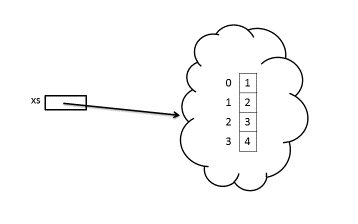
\includegraphics[scale=1.2]{../img/w05-solutions/memory-pic-2}
\item 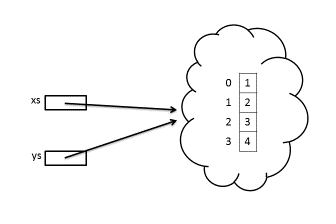
\includegraphics[scale=1.2]{../img/w05-solutions/memory-pic-3}
\item 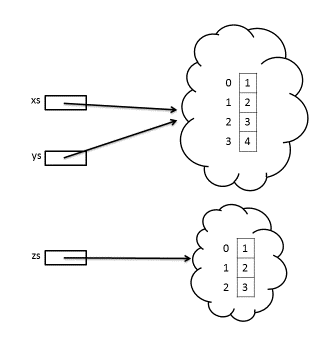
\includegraphics[scale=1.2]{../img/w05-solutions/memory-pic-4}
\item 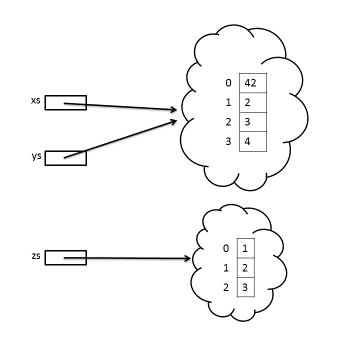
\includegraphics[scale=1.2]{../img/w05-solutions/memory-pic-5}
\item 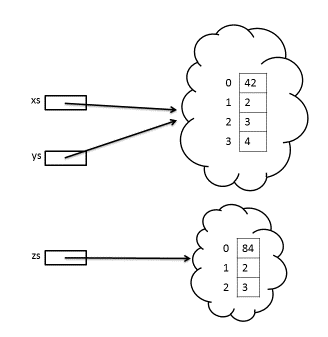
\includegraphics[scale=1.2]{../img/w05-solutions/memory-pic-6}
\end{enumerate}
xs = Array(42, 2, 3, 4)\\
ys = Array(42, 2, 3 ,4)\\
zs = Array(84, 2, 3)\\
\code{xs} och \code{yx} refererar till samma objekt och då deras första IntCell:s värde ändras till 42, så kommer förändringen att ske för båda.
\code{zs} har en referens till ett annat objekt med ett mindre element. Att \code{zs}:s första element ändras, påverkar inte \code{xs} och \code{ys}.



\QUESTEND




%%<AUTOEXTRACTED by mergesolu>%%      % Uppgift 5




\WHAT{Algoritm: SEQ-REVERSE-COPY.}

\QUESTBEGIN

\Task  \what~  Implementera nedan algoritm:

\begin{algorithm}[H]
 \SetKwInOut{Input}{Indata}\SetKwInOut{Output}{Resultat}

 \Input{Heltalsarray $xs$}
 \Output{En ny heltalsarray med elementen i $xs$ i omvänd ordning.}
 $n \leftarrow$ antalet element i $xs$ \\
 $ys \leftarrow$ en ny heltalsarray med plats för $n$ element\\
 $i \leftarrow 0$  \\
 \While{$i < n$}{
  $ys(n - i - 1) \leftarrow xs(i)$ \\
  $i \leftarrow i + 1$
 }
 \Return $ys$
\end{algorithm}

\Subtask\Pen Skriv implementation med penna och papper. Använd en \code{while}-sats på samma sätt som i algoritmen. Prova sedan din implementation på dator och kolla så att den fungerar.

\Subtask\Pen \label{subtask:for-seq-copy} Skriv implementationen med penna och papper igen, men använd nu istället en \code{for}-sats som räknar baklänges. Prova sedan din implementation på dator och kolla så att den fungerar.

\Subtask Definiera en funktion i REPL med namnet \code{reverseCopy} med din implementation i uppgift \ref{subtask:for-seq-copy}.


\SOLUTION


\TaskSolved \what
 

\SubtaskSolved  \begin{Code}
def seqReverseCopy(xs: Array[Int]): Array[Int] = {
  val n = xs.size
  val ys = Array.fill[Int](n)(0)
  var i = 0
  while(i < n) {
    ys(n-i-1) = xs(i)
    i += 1
  }
  ys
}
\end{Code}

\SubtaskSolved  \begin{Code}
def seqReverseCopy(xs: Array[Int]): Array[Int] = {
  val n = xs.size
  val ys = Array.fill[Int](n)(0)
  for(i <- n-1 to 0 by -1) ys(n-i-1) = xs(i)
  ys
}
\end{Code}

\SubtaskSolved  Se b).



\QUESTEND




%%<AUTOEXTRACTED by mergesolu>%%      % Uppgift 6




\WHAT{Algoritm: SEQ-REVERSE.}

\QUESTBEGIN

\Task  \what~  Strängar av typen \code{String} är oföränderliga. Vill man ändra i en sträng utan att skapa en ny kopia kan man använda en \code{StringBuilder} enligt nedan algoritm som vänder bak-och-fram på en sträng.

\begin{algorithm}[H]
 \SetKwInOut{Input}{Indata}\SetKwInOut{Output}{Resultat}

 \Input{En sträng $s$ av typen \texttt{String}}
 \Output{En ny sträng av typen \texttt{String}}
 $sb \leftarrow$ en ny \texttt{StringBuilder} som innehåller $s$ \\
 $n \leftarrow$ antalet tecken i $s$\\
 \For{$i \leftarrow 0$ \KwTo $\frac{n}{2} - 1$}{
  $temp \leftarrow sb(i)$ \\
  $sb(i) \leftarrow sb(n - i - 1)$ \\
  $sb(n - i - 1) \leftarrow temp$ \\
 }
 \Return $sb$ omvandlad till en \texttt{String}
\end{algorithm}

\Subtask Implementera algoritmen ovan i en funktion med signaturen: \\
 \code{def reverseString(s: String): String}

\Subtask Använd din funktion \code{reverseString} från föregående deluppgift i en ny funktion med signaturen:\\
 \code{def isPalindrome(s: String): Boolean} \\ som avgör om en sträng är en palindrom.\footnote{\href{https://sv.wikipedia.org/wiki/Palindrom}{sv.wikipedia.org/wiki/Palindrom}}

\Subtask\Pen Man kan med en \code{while}-sats och indexering direkt i en \code{String} avgöra om en sträng är en palindrom utan att kopiera den till en \code{StringBuilder}. Implementera en ny variant av \code{isPalindrome} som använder denna metod. Skriv först algoritmen på papper i pseudo-kod.

\SOLUTION


\TaskSolved \what
 

\SubtaskSolved  \begin{Code}
def reverseString(s: String): String = {
  val sb = new StringBuilder(s)
  val n = sb.length
  for (i <- 0 until n / 2) {
    val temp = sb(i)
    sb(i) = sb(n - i - 1)
    sb(n - i - 1) = temp
  }
  sb.toString
}
\end{Code}

\SubtaskSolved  \begin{Code}
def isPalindrome(s: String): Boolean = {s == reverseString(s)}
\end{Code}

\SubtaskSolved  \begin{Code}
def isPalindrome(s: String): Boolean = {
  val n = s.length
  var foundDiff = false
  var i = 0
  while (i < n/2 && !foundDiff)  {
    foundDiff = s(i) != s(n - i - 1)
    i += 1
  }
  !foundDiff
}
\end{Code}



\QUESTEND




%%<AUTOEXTRACTED by mergesolu>%%      % Uppgift 7




\WHAT{Algoritm: SEQ-REGISTER.}

\QUESTBEGIN

\Task \label{task:seq-reg} \what~   Algoritmer för registrering löser problemet att räkna förekomst av olika saker, till exempel antalet tärningskast som gav en sexa. Antag att vi har följande vektor \code{xs} som representerar 13 st tärningskast:
\begin{REPL}
scala> val xs = Vector(5, 3, 1, 6, 1, 3, 5, 1, 1, 6, 3, 2, 6)
\end{REPL}
\Subtask Använd metoderna \code{filter} och \code{size} på \code{xs} för att filtrera ut alla 6:or och räkna hur många de är.

\Subtask Använd metoderna \code{filter} och \code{size} på \code{xs} för att filtrera ut alla jämna kast och räkna hur många de är.

\Subtask Metoden \code{groupBy} på en samling tar en funktion \code{f} som parameter och skapar en ny \code{Map} med nycklar \code{k} som är associerade till samlingar som utgör grupper av värden där
\code{f(x) == k}.  Vad händer här:
\begin{REPL}
scala> xs.groupBy(x => x % 2)
scala> xs.groupBy(_ % 2)
scala> xs.groupBy(_ % 3)
scala> xs.groupBy(_ % 3).foreach(println)
scala> val freqEvenOdd = xs.groupBy(_ % 2).map(p => (p._1, p._2.size))
scala> val nEven = freqEvenOdd(0)
scala> val nOdd = freqEvenOdd(1)
\end{REPL}
\Subtask Använd metoden \code{groupBy} på \code{xs} med den s.k. identitetsfunktionen \code{i => i} som returnerar sitt eget argument. Vad händer?

\Subtask Definiera en \code{val freq: Map[Int, Int]} som räknar antalet olika tärningsutfall i \code{xs}. Använd metoden \code{groupBy} på \code{xs} med identitetsfunktionen följt av en \code{map} med funktionen \code{p => (p._1, p._2.size)}.

\Subtask Du ska nu själv implementera en registreringsalgoritm. Skriv en funktion:
\begin{Code}
def tärningsRegistrering(xs: Array[Int]): Array[Int] = ???
\end{Code}
som implementerar nedan algoritm (som alltså inte använder \code{groupBy} eller andra färdiga metoder på samlingar förutom \code{size} och \code{apply}).

\begin{algorithm}[H]
 \SetKwInOut{Input}{Indata}\SetKwInOut{Output}{Resultat}

 \Input{En array $xs$ med heltal mellan 1 och 6 som representerar utfall av många tärningskast.}
 \Output{En array $f$ med 7 st element där $f(0)$ innehåller totala antalet kast, $f(1)$ anger antalet ettor, $f(2)$ antalet tvåor, etc. till och med $f(6)$ som anger antalet sexor.}
 $f \leftarrow$ en ny array med $7$ element där alla element initaliseras till 0.\\
 $f(0) \leftarrow$ antalet element i $xs$ \\
 $i \leftarrow 0$  \\
 \While{$i < f(0)$}{
  $f(xs(i)) \leftarrow f(xs(i)) + 1$ \\
  $i \leftarrow i + 1$
 }
 \Return $f$
\end{algorithm}

Testa din funktion med nedan funktionsanrop:
\begin{REPL}
scala> tärningsRegistrering(Array.fill(1000)((math.random * 6).toInt + 1))
res12: Array[Int] = Array(1000, 174, 174, 167, 171, 145, 169)
\end{REPL}

\SOLUTION


\TaskSolved \what
 

\SubtaskSolved  \code{xs.filter(_ == 6).size}

\SubtaskSolved  \code{xs.filter(_ % 2 == 0).size}

\SubtaskSolved  \begin{REPL}
scala.collection.immutable.Map[Int,scala.collection.immutable.Vector[Int]] =
	Map(1 -> Vector(5, 3, 1, 1, 3, 5, 1, 1, 3), 0 -> Vector(6, 6, 2, 6))
scala.collection.immutable.Map[Int,scala.collection.immutable.Vector[Int]] =
	Map(1 -> Vector(5, 3, 1, 1, 3, 5, 1, 1, 3), 0 -> Vector(6, 6, 2, 6))
scala.collection.immutable.Map[Int,scala.collection.immutable.Vector[Int]] =
	Map(2 -> Vector(5, 5, 2), 1 -> Vector(1, 1, 1, 1), 0 -> Vector(3, 6, 3, 6, 3, 6))
(2,Vector(5, 5, 2))
(1,Vector(1, 1, 1, 1))
(0,Vector(3, 6, 3, 6, 3, 6))
freqEvenOdd: scala.collection.immutable.Map[Int,Int] = Map(1 -> 9, 0 -> 4)
nEven: Int = 4
nOdd: Int = 9
\end{REPL}

\SubtaskSolved  \code{xs.groupBy(i => i)} skapar en map där nycklarna är alla unika element och värdena är av samma värde som respektive nyckel.

\SubtaskSolved  \code{val freq: Map[Int, Int] = xs.groupBy(i => i).map(p => (p._1, p._2.size))}

\SubtaskSolved  \begin{Code}
def tärningsRegistrering(xs: Array[Int]): Array[Int] = {
  val f = Array.fill(7)(0)
  f(0) = xs.size
  var i = 0
  while (i < f(0)) {
    f(xs(i)) += 1
    i += 1
  }
  f
}
\end{Code}



\QUESTEND




%%<AUTOEXTRACTED by mergesolu>%%      % Uppgift 8




\WHAT{Algoritm: SEQ-REMOVE-COPY.}

\QUESTBEGIN

\Task  \what~  Ibland vill man kopiera alla element till en ny \code{Array} \emph{utom} ett element på en viss plats \code{pos}.

\Subtask\Pen Skriv algoritmen SEQ-REMOVE-COPY i pseudokod med penna på papper.

\Subtask Implementera algoritmen SEQ-REMOVE-COPY i en funktion med denna signatur:
\begin{Code}
def removeCopy(xs: Array[Int], pos: Int): Array[Int]
\end{Code}

\SOLUTION


\TaskSolved \what
 

\SubtaskSolved 

\begin{algorithm}[H]
 \SetKwInOut{Input}{Indata}\SetKwInOut{Output}{Resultat}

 \Input{En sekvens $xs$ av typen \texttt{Array[Int]} och $pos$}
 \Output{En ny sekvens av typen \texttt{Array[Int]} som är en kopia av $xs$ fast med elementet på plats $pos$ borttaget}
 $n \leftarrow$ antalet element $xs$\\
 $ys \leftarrow$ en ny \texttt{Array[Int]} med plats för $n-1$ element \\
 \For{$i \leftarrow 0$ \KwTo $pos - 1$}{
  $ys(i) \leftarrow xs(i)$
 }
 $ys(pos) \leftarrow x$ \\
 \For{$i \leftarrow pos+1$ \KwTo $n - 1$}{
  $ys(i - 1) \leftarrow xs(i)$
 }
 \Return $ys$
\end{algorithm}

\SubtaskSolved  \begin{Code}
def removeCopy(xs: Array[Int], pos: Int): Array[Int] = {
  val n = xs.size
  val ys = Array.fill(n - 1)(0)
  for (i <- 0 until pos) ys(i) = xs(i)
  for (i <- pos+1 until n) ys(i - 1) = xs(i)
  ys
}
\end{Code}



\QUESTEND




%%<AUTOEXTRACTED by mergesolu>%%      % Uppgift 9




\WHAT{Algoritm: SEQ-REMOVE.}

\QUESTBEGIN

\Task  \what~  Ibland vill man ta bort ett element på en viss position i en befintlig \code{Array} utan att kopiera alla element till en ny \code{Array}. Ett sätt att göra detta är att flytta alla efterföljande element ett steg mot lägre index och låta sista platsen bli 0.

\Subtask\Pen Skriv algoritmen SEQ-REMOVE i pseudokod med penna på papper.

\Subtask Implementera algoritmen SEQ-REMOVE i en funktion med denna signatur:
\begin{Code}
def remove(xs: Array[Int], pos: Int): Unit
\end{Code}


%%%%%%%%%%%%%%%%%%%%%%%%%%%%%%%%%%%%%%%%%%%5


\SOLUTION


\TaskSolved \what
 

\SubtaskSolved 

\begin{algorithm}[H]
 \SetKwInOut{Input}{Indata}\SetKwInOut{Output}{Resultat}

 \Input{En sekvens $xs$ av typen \texttt{Array[Int]} och $pos$}
 \Output{En uppdaterad sekvens av $xs$ där elementet på plats $pos$ tagits bort och efterföljande element flyttas ett steg mot lägre index med ett sista elementet som är $0$}
 $n \leftarrow$ antalet element $xs$\\
 \For{$i \leftarrow pos+1$ \KwTo $n - 1$}{
  $xs(i - 1) \leftarrow xs(i)$
 }
 $xs(n - 1) \leftarrow 0$ \\
\end{algorithm}

\SubtaskSolved  \begin{Code}
def remove(xs: Array[Int], pos: Int): Unit = {
  val n = xs.size
  for (i <- pos+1 until n) xs(i - 1) = xs(i)
  xs(n-1) = 0
}
\end{Code}



\QUESTEND




%%<AUTOEXTRACTED by mergesolu>%%      % Uppgift 10




\WHAT{Deterministiska pseudoslumptalssekvenser med \code{java.util.Random}.}

\QUESTBEGIN

\Task  \what~  Klassen \code{java.util.Random} ger möjlighet att generera en sekvens av tal som verkar slumpmässiga. Genom att välja ett visst s.k. \textbf{frö} \Eng{seed} kan man få samma sekvens av pseudoslumptal varje gång.

\Subtask\Pen Sök upp och studera dokumentationen för \code{java.util.Random}. Hur skapar man en ny instans av klassen \code{Random}? Vad gör operationen \code{nextInt} på \code{Random}-objekt.

\Subtask Förklara vad som händer nedan?
\begin{REPL}
scala> import java.util.Random
scala> val frö = 42L
scala> val rnd = new Random(frö)
scala> rnd.nextInt(10)
scala> (1 to 100).foreach(_ => print(rnd.nextInt(10)))
scala> val rnd1 = new Random(frö)
scala> val rnd2 = new Random(frö)
scala> val rnd3 = new Random(System.nanoTime)
scala> val rnd4 = new Random((math.random * Long.MaxValue).toLong)
scala> def flip(r: Random) = if (r.nextInt(2) > 0) "krona" else "klave"
scala> val xs = (1 to 100).map{i =>
			(flip(rnd1), flip(rnd2), flip(rnd3), flip(rnd4))}
scala> xs foreach println
scala> xs.exists(q => q._1 != q._2)
scala> xs.exists(q => q._1 != q._3)
\end{REPL}

\Subtask\Pen Nämn några sammanhang då det är användbart att kunna bestämma fröet till en slumptalssekvens.

\Subtask Blir det samma sekvens om du använder fröet \code{42L} som argument till konstruktorn vid skapandet av en instans av \code{java.util.Random} på en \emph{annan} dator?

\Subtask Sök reda på dokumentationen för \code{java.math.random} och undersök hur denna sekvens skapas.

\Subtask Vad blir det för frö till slumptalssekvensen om man skapar ett \code{Random}-objekt med hjälp av konstruktorn utan parameter?

\SOLUTION


\TaskSolved \what
 

\SubtaskSolved  Antingen kan du skapa en ny instans av \code{java.util.Random} genom att skriva: \code{val r1 = new java.util.Random}.
Men om \code{java.util.Random} importeras kan “java.util” skippas och istället skrivs: \code{val r2 = new Random}.
Som valfritt argument kan ett slumptalsfrö av typen Long skickas med när en ny instans skapas, e.g. \code{val r3 = new Random(42L)}.
\code{nextInt(x)} skapar ett slumptal från och med 0, upp till x (exklusive x).

\SubtaskSolved  \begin{REPL}
import java.util.Random // Importerar Random

frö: Long = 42 // Ett slumptalsfrö av värdet 42L skapas.

  // Skapar ett Random objekt med slumptalsfrö "frö".
rnd: java.util.Random = java.util.Random@2f410acf

res0: Int = 7 // Slumpade fram ett tal från 0 till och med 9.

9 8 8 8 9 7 2 1 4 0 0 3 8 8 4 5 9 1 3 3 5 1 1
3 3 3 6 3 4 7 5 7 8 7 6 9 7 0 3 0 6 6 1 0 8 1
1 1 0 5 3 5 1 5 3 5 9 9 5 1 8 9 0 6 4 7 5 7 9
6 4 0 8 1 0 9 6 6 3 2 7 9 2 7 0 6 9 8 5 0 0 8
9 2 7 7 3 5 1 3 // Slumpar och skriver ut 100 tal från 0 till och med 9.

  // Skapar ett Random objekt med slumptalsfrö "frö".
rnd1: java.util.Random = java.util.Random@31e4bb20

  // Skapar ett Random objekt med slumptalsfrö "frö".
rnd2: java.util.Random = java.util.Random@45e37a7e

  // Skapar ett Random objekt med slumptalsfrö med
  // värdet av vad tiden är just nu i nanosekunder.
rnd3: java.util.Random = java.util.Random@57eda880

  // Skapar ett Random objekt med slumptalsfrö
  // med värdet (math.random * Long.MaxValue).toLong.
rnd4: java.util.Random = java.util.Random@79da1ec0

flip: (r: java.util.Random)String // Skapar en funktion som singlar slant.

  // Singlar slant med alla fyra Random
  // objekt 100 gånger samt printar ut resultatet.
xs: scala.collection.immutable.IndexedSeq[(String, String, String, String)] =
Vector((krona,krona,krona,klave), (klave,klave,krona,krona), (krona,krona,klave,klave),
(klave,klave,krona,klave), (klave,klave,krona,krona), (krona,krona,klave,krona),
(klave,klave,klave,klave), (krona,krona,klave,krona), (krona,krona,klave,krona),
(klave,klave,krona,klave), (krona,krona,krona,klave), (klave,klave,krona,klave),
(klave,klave,krona,krona), (klave,klave,klave,krona), (klave,klave,klave,krona),
(krona,krona,klave,klave), (klave,klave,klave,klave), (krona,krona,klave,krona),
(krona,krona,klave,klave), (krona,krona,klave,klave), (krona,krona,klave,krona),
(klave,klave,klave,klave), (klave,klave,krona,krona), (klave,klave,klave,klave),
(krona,krona,krona,krona), (krona,krona,krona,klave)...

  // Kollar om det finns något värde som rnd1
  // har genererat men som inte rnd2 genererat.
res1: Boolean = false

  // Kollar om det finns något värde som rnd1
  // har genererat men som inte rnd3 genererat.
res2: Boolean = true

\end{REPL}

\SubtaskSolved  Vid felsökning och vid simulering där man vill att samma “slumpmässiga” sekvens uppstår varenda gång.

\SubtaskSolved  Ja.

\SubtaskSolved  \url{https://docs.oracle.com/javase/7/docs/api/java/lang/Math.html#random%28%29--} säger att den skapar ett nytt java.util.Random-objekt.

\SubtaskSolved  Den skapar ett slumpmässigt slumptalsfrö. För mer information, se: \url{https://docs.oracle.com/javase/8/docs/api/java/util/Random.html#Random--}



\QUESTEND




%%<AUTOEXTRACTED by mergesolu>%%      % Uppgift 11




\WHAT{Undersök om tärningskast är rektangelfördelade.}

\QUESTBEGIN

\Task  \what~ \footnote{För ett rektangelfördelat slumpvärde gäller att om man drar (nästan oändligt många) slumpvärden så blir det (nästan) lika många av varje möjligt värde. Om man ritar en sådan fördelning i ett koordinatsystem med antalet utfall på y-axeln och de olika värdena på x-axeln, så blir bilden rektangelformad. Du får lära dig mer om sannolikhetsfördelningar i kommande kurser i matematisk statistik.} \\Skriv en funktion \code{def testRandom(r: Random, n: Int): Unit = ???} \\ som ger följande utskrift:
\begin{REPL}
scala> val rnd = new Random(42L)
scala> testRandom(rnd, 1000)
Antal kast: 1000
Antal 1:or: 178
Antal 2:or: 187
Antal 3:or: 167
Antal 4:or: 148
Antal 5:or: 155
Antal 6:or: 165
\end{REPL}

\emph{Tips:}
Anropa din funktion \code{tärningsRegistrering} från uppgift \ref{task:seq-reg}.


\SOLUTION


\TaskSolved \what
 

\begin{Code}
def testRandom(r: Random, n: Int): Unit = {
  val xs = Array.fill(n)(r.nextInt(6) + 1)
  val f = tärningsRegistrering(xs)
  println("Antal kast: " + f(0))
  for (i <- 1 to 6) println(s"Antal $i:or: " + f(i))
}
\end{Code}



\QUESTEND




%%<AUTOEXTRACTED by mergesolu>%%      % Uppgift 12




\WHAT{Array och \code{for}-sats i Java.}

\QUESTBEGIN

\Task  \what~ 

\Subtask Skriv nedan program i en editor och spara i filen \code{DiceReg.java}:

\javainputlisting{examples/DiceReg.java}

\Subtask Kompilera med \code{javac DiceReg.java} och kör med \code{java DiceReg 10000 42} och förklara vad som händer.

\Subtask\Pen Beskriv skillnaderna mellan Scala och Java, vad gäller syntaxen för array och \code{for}-sats. Beskriv några andra skillnader mellan språken som syns i programmet ovan.

\Subtask Ändra i programmet ovan så att loop-variabeln \code{i} skrivs ut i varje runda i varje \code{for}-sats. Kompilera om och kör.

\Subtask Skriv om programmet ovan genom att abstrahera huvudprogrammets delar till de statiska metoderna \code{parseArguments}, \code{registerPips} och \code{printReg} enligt nedan skelett. Notera speciellt hur \jcode{private} och \jcode{public} är angivet. Spara programmet i filen \code{DiceReg2.java} och kompilera med \texttt{javac DiceReg2.java} i terminalen.

\begin{Code}[language=Java]
// DiceReg2.java
import java.util.Random;

public class DiceReg2 {
    public static int[] diceReg = new int[6];
    private static Random rnd = new Random();

    public static int parseArguments(String[] args) {
        // ???
        return n;
    }

    public static void registerPips(int n){
        // ???
    }

    public static void printReg() {
        // ???
    }

    public static void main(String[] args) {
        int n = parseArguments(args);
        registerPips(n);
        printReg();
    }
}
\end{Code}

\Subtask Starta Scala REPL i samma bibliotek som filen \texttt{DiceReg2.class} ligger i och kör nedan satser och förklara vad som händer:
\begin{REPL}
scala> DiceReg2.main(Array("1000","42"))
scala> DiceReg2.diceReg
scala> DiceReg2.registerPips(1000)
scala> DiceReg2.printReg
scala> DiceReg2.registerPips(1000)
scala> DiceReg2.printReg
scala> DiceReg2.rnd
\end{REPL}

\Subtask Växla synligheten på attributen mellan \jcode{private} och \jcode{public}, kompilera om och studera effekten i Scala REPL. Hur lyder felmeddelandet om du försöker komma åt en privat medlem?

\Subtask\Pen Ange en viktig anledning till att man kan vilja göra medlemmar privata.



\SOLUTION


\TaskSolved \what
 

\SubtaskSolved  -

\SubtaskSolved  \begin{REPL}
Rolling the dice 10000 times with seed 42
Number of 1's: 1654
Number of 2's: 1715
Number of 3's: 1677
Number of 4's: 1629
Number of 5's: 1643
Number of 6's: 1682
\end{REPL}
Simulerar 10000 tärningskast (med slumptalsfrö 42) och skriver ut förekomsten av respektive tärningskast.

\SubtaskSolved  Array i scala deklararas: \code{val scalaArray = Array.ofDim[Int](6)} medan i java skrivs: \code{int[] javaArray = new int[6];}
\code{for}-sats i scala skrivs: \code{for(i <- 0 to n)} medan i java skrivs: \code{for (int i = 0; i < n; i++)}.
I java måste semicolon skrivas efter varje operation samt att typen måste explicit definieras vid variabeldeklaration.
I scala behövs inga semicolon (förutom för att separera operationer på samma rad) och scala bestäms typen implicit, alltså att kompilatorn “gissar” typen av variabeln som deklareras.

\SubtaskSolved  Lägg till \code{System.out.println(i);} i for-looparna

\SubtaskSolved  \begin{Code}[language=Java]
// DiceReg2.java
import java.util.Random;
public class DiceReg2{
	public static int[] diceReg = new int[6];
	private static Random rnd = new Random();

	public static int parseArguments(String[] args){
		int n = 100;
		if(args.length > 0) {
			n = Integer.parseInt(args[0]);
		}
		if(args.length > 1) {
			int seed = Integer.parseInt(args[1]);
			rnd.setSeed(seed);
		}
		return n;
	}

	public static void registerPips(int n) {
		for(int i = 0; i<n; i++) {
			int pips = rnd.nextInt(6);
			diceReg[pips]++;
		}
	}

	public static void main(String[] args) {
		int n = parseArguments(args);
		registerPips(n);
		printReg();
	}
}
\end{Code}

\SubtaskSolved  \begin{REPL}
  // Skriver ut förekomsten av 1000 tärningskast med slumptalsfrö 42.
Number of 1's: 165
Number of 2's: 163
Number of 3's: 178
Number of 4's: 183
Number of 5's: 156
Number of 6's: 155

  // Skriver ut diceReg-attributet
res1: Array[Int] = Array(165, 163, 178, 183, 156, 155)

  // Skriver ut diceReg-attributet efter 1000 till kast.
res2: Array[Int] = Array(329, 325, 349, 360, 324, 313)

  // Skriver ut diceReg-attributet efter 1000 till kast.
res3: Array[Int] = Array(498, 484, 531, 513, 485, 489)

  // Det blir runtime error då attributet rnd är
  // private och kan inte nås via REPL:n.
<console>:11: error: value rnd is not a member of object DiceReg2
	DiceReg2.rnd
				    ^
\end{REPL}

\SubtaskSolved  \begin{REPL}
value [diceReg/rnd] is not a member of object DiceReg2
\end{REPL}

\SubtaskSolved  Om man ska spara under någon data som man inte vill att användaren, eller någon annan, inte ska kunna komma åt.
T.ex. om du gör en bankapp vill du inte att nyckeln som du använder för att autorisera en användare ska vara tillgänglig för då kan hackare använda det för att ta sig in på kontot och stjäla pengar!



\QUESTEND




%%<AUTOEXTRACTED by mergesolu>%%      % Uppgift 13




\WHAT{Läsa in tal med \code{java.util.Scanner}.}

\QUESTBEGIN

\Task  \what~  Med \jcode{new Scanner(System.in)} skapas ett objekt som kan läsa in tal som användaren skriver i terminalfönstret.

\Subtask Sök upp och studera dokumentationen för \code{java.util.Scanner}. Vad gör metoderna \jcode{hasNextInt()} och \jcode{nextInt()}?

\Subtask Skriv nedan program i en editor och spara i filen \code{DiceScanBuggy.java}:

\javainputlisting{examples/DiceScanBuggy.java}

\Subtask Kompilera och kör med indatasekvensen \texttt{1 2 3 4 -1} och notera hur registreringen sker.

\Subtask Programmet fungerar inte som det ska. Du behöver korrigera 3 saker för att programmet ska göra rätt. Rätta buggarna och spara det rättade programmet som \texttt{DiceScan.java}. Kompilera och testa att det rättade programmet fungerar med olika indata.


\SOLUTION


\TaskSolved \what
 

\SubtaskSolved  \code{hasNextInt()} kollar enbart om det finns ett till tal och returnerar \code{true}/\code{false}. \code{nextInt()} “hoppar” till nästa tal och returnerar det.
Se \url{https://docs.oracle.com/javase/7/docs/api/java/util/Scanner.html#hasNextInt%28%29} och \url{https://docs.oracle.com/javase/7/docs/api/java/util/Scanner.html#nextInt%28%29 }.

\SubtaskSolved  -

\SubtaskSolved  -

\SubtaskSolved  \begin{Code}[language=Java,numbers=left]
import java.util.Random;
import java.util.Scanner;

public class DiceScanBuggy {
	public static int[] diceReg = new int[6];
	public static Scanner scan = new Scanner(System.in);

	public static void registerPips() {
		System.out.println("Enter pips separated by blanks: ");
		System.out.println("End with -1 and <Enter>.");
		boolean isPips = true;
		while(isPips && scan.hasNextInt()){
			int pips = scan.nextInt();
			if(pips >= 1 && pips <= 6) {
				diceReg[pips-1]++;
			} else {
				isPips = false;
			}
		}
	}

	public static void printReg(){
		for(int i = 1; i<7; i++) {
		System.out.println("Number of " + i + "'s: " + diceReg[i-1]);
		}
	}

	public static void main(String[] args) {
		registerPips();
		printReg();
	}
}
\end{Code}


\QUESTEND




%%<AUTOEXTRACTED by mergesolu>%%      % Uppgift 14




\WHAT{Välja sekvenssamling.}

\QUESTBEGIN

\Task  \what~\Pen  Vilken av \code{Vector}, \code{Array} och \code{ArrayBuffer} hade du valt i dessa situationer?

\Subtask Ditt program innehåller en sekvens av objekt med data om alla ca $10^7$ medborgare i Sverige. Efter noggranna mätningar visar det sig att tillägg av objekt på godtyckliga ställen i sekvensen är en flaskhals.

\Subtask Ditt program innehåller en sekvens av objekt med data om ca $10^2$ \href{https://sv.wikipedia.org/wiki/Residensstad#Sverige}{residensstäder} i Sverige. Senast det skedde en uppdatering av mängden referensstäder var 1997. Prestandamätningar visar att det är uppdatering av attributvärden i objekten som tar mest tid. Städerna behöver kunna bearbetas i godtycklig ordning.

\Subtask Ditt program innehåller en sekvens av ca $10^9$ osorterade heltal som ska läsas in från fil och sorteras på plats i minnet. Det första talet i filen anger antalet heltal. Det är viktigt att sorteringen går snabbt. När talen är sorterade ska de skrivas tillbaka till fil i sorterad ordning.

\Subtask Ditt program innehåller en sekvens av ett känt antal oföränderliga objekt med data om genomförda banktransaktioner. Sekvensen ska bearbetas parallellt i godtycklig ordning med olika algoritmer som kan köras oberoende av varandra.


\ExtraTasks %%%%%%%%%%%%%%%%%%%

\SOLUTION


\TaskSolved \what
 

\SubtaskSolved  \code{ArrayBuffer}.

\SubtaskSolved  \code{ArrayBuffer} eller \code{Array}.

\SubtaskSolved  \code{Array}.

\SubtaskSolved  \code{Vector}.



\ExtraTasks %%%%%%%%%%%%


\QUESTEND




%%<AUTOEXTRACTED by mergesolu>%%      % Uppgift 15




\WHAT{Algoritm: SEQ-INSERT-COPY.}

\QUESTBEGIN

\Task  \what~ 

\begin{algorithm}[H]
 \SetKwInOut{Input}{Indata}\SetKwInOut{Output}{Resultat}

 \Input{En sekvens $xs$ av typen \texttt{Array[Int]} och heltalen $x$ och $pos$}
 \Output{En ny sekvens av typen \texttt{Array[Int]} som är en kopia av $xs$ men där $x$ är infogat på plats $pos$}
 $n \leftarrow$ antalet element $xs$\\
 $ys \leftarrow$ en ny \texttt{Array[Int]} med plats för $n+1$ element \\
 \For{$i \leftarrow 0$ \KwTo $pos - 1$}{
  $ys(i) \leftarrow xs(i)$
 }
 $ys(pos) \leftarrow x$ \\
 \For{$i \leftarrow pos$ \KwTo $n - 1$}{
  $ys(i + 1) \leftarrow xs(i)$
 }
 \Return $ys$
\end{algorithm}

\Subtask Implementera ovan algoritm i en funktion med denna signatur:
\begin{Code}
def insertCopy(xs: Array[Int], x: Int, pos: Int): Array[Int]
\end{Code}

\Subtask Vad måste \code{pos} vara för att det ska fungera med en tom array som argument?

\Subtask Vad händer om din funktion anropas med ett negativt argument för \code{pos}?

\Subtask Vad händer om din funktion anropas med \code{pos} lika med \code{xs.size}?

\Subtask Vad händer om din funktion anropas med \code{pos} större än \code{xs.size}?



\SOLUTION


\TaskSolved \what
 

\SubtaskSolved  \begin{Code}
def insertCopy(xs: Array[Int], x: Int, pos: Int): Array[Int] = {
  val n = xs.size
  val ys = Array.ofDim[Int](n + 1)
  for (i <- 0 until pos) ys(i) = xs(i)
  ys(pos) = x
  for (i <- pos until n) ys(i + 1) = xs(i)
  ys
}
\end{Code}

\SubtaskSolved  \code{pos} måste vara \code{0}.

\SubtaskSolved  \begin{REPL}
java.lang.ArrayIndexOutOfBoundsException: -1
\end{REPL}

\SubtaskSolved  Elementet \code{x} läggs till på slutet av arrayen, alltså kommer den returnerande arrayen vara större än den som skickades in.

\SubtaskSolved  \begin{REPL}
java.lang.ArrayIndexOutOfBoundsException: 5
\end{REPL}
Man får \code{ArrayIndexOutOfBoundsException} då indexeringen är utanför storleken hos arrayen.


\QUESTEND




%%<AUTOEXTRACTED by mergesolu>%%      % Uppgift 16




\WHAT{Algoritm: SEQ-INSERT.}

\QUESTBEGIN

\Task  \what~  Man kan implementera algoritmen SEQ-INSERT på plats i en \code{Array[Int]} så att alla elementen efter \code{pos} flyttas fram ett steg och att sista elementet ''försvinner''.

\Subtask\Pen Skriv algoritmen SEQ-INSERT i pseudokod med penna och papper.

\Subtask Implemtera SEQ-INSERT i en funktion med denna signatur:
\begin{Code}
def insert(xs: Array[Int], x: Int, pos: Int): Unit
\end{Code}

\SOLUTION


\TaskSolved \what
 

\SubtaskSolved 

\begin{algorithm}[H]
 \SetKwInOut{Input}{Indata}\SetKwInOut{Output}{Resultat}

 \Input{En sekvens $xs$ av typen \texttt{Array[Int]} och heltalen $x$ och $pos$}
 \Output{En uppdaterad sekvens av $xs$ där elementet $x$ har satts in på platsen $pos$ och efterföljande element flyttas ett steg där sista elementet försvinner}
 $n \leftarrow$ antalet element $xs$\\
 $ys \leftarrow$ en klon av $xs$\\
 $xs(pos) \leftarrow x$\\
 \For{$i \leftarrow pos+1$ \KwTo $n - 1$}{
  $xs(i) \leftarrow ys(i - 1)$
 }
\end{algorithm}

\SubtaskSolved  \begin{Code}
def insert(xs: Array[Int], x: Int, pos: Int): Unit = {
  val n = xs.size
  val ys = xs.clone
  xs(pos) = x
  for (i <- pos + 1 until n) xs(i) = ys(i - 1)
}
\end{Code}



\QUESTEND




%%<AUTOEXTRACTED by mergesolu>%%      % Uppgift 17




\WHAT{NEEDS A TOPIC DESCRIPTION}

\QUESTBEGIN

\Task  \what~ Implementera funktionen \code{tärningsRegistrering} från uppgift \ref{task:seq-reg} på nytt, men nu med en \code{for}-sats istället.


\SOLUTION


\TaskSolved \what
 

\begin{Code}
def tärningsRegistrering(xs: Array[Int]): Array[Int] = {
  val f = Array.fill(7)(0)
  f(0) = xs.size
  for(i <- 0 until f(0)) f(xs(i)) += 1
  f
}
\end{Code}



\QUESTEND




%%<AUTOEXTRACTED by mergesolu>%%      % Uppgift 18




\WHAT{NEEDS A TOPIC DESCRIPTION}

\QUESTBEGIN

\Task  \what~ Bygg vidare på Keno-uppgiften nummer \ref{task:keno-set} i kapitel \ref{chapter:W04} på sidan \pageref{task:keno-set} och gör registrering av det slumpmässiga utfallet av 365 Keno-dragningar och skriv ut frekvenserna för förekomsten av varje boll. Öka sedan antalet dragningar och undersök hur många dragningar du behöver göra för att frekvenserna ska bli nästan lika?


\AdvancedTasks %%%%%%%%%%%%%%%%%

\SOLUTION


\TaskSolved \what
 



\AdvancedTasks %%%%%%%%%



\QUESTEND




%%<AUTOEXTRACTED by mergesolu>%%      % Uppgift 19




\WHAT{NEEDS A TOPIC DESCRIPTION}

\QUESTBEGIN

\Task  \what~ Sök reda på dokumentationen för metoden \code{patch} på klassen \code{Array}.

\Subtask Använd metoden \code{patch} för att implementera SEQ-INSERT-COPY:
\begin{Code}
def insertCopy(xs: Array[Int], x: Int, pos: Int): Array[Int] =
  xs.patch(???, ???, ???)
\end{Code}

\Subtask Använd metoden \code{patch} för att  implementera SEQ-REMOVE-COPY:
\begin{Code}
def removeCopy(xs: Array[Int], pos: Int): Array[Int] =
  xs.patch(???, ???, ???)
\end{Code}

\SOLUTION


\TaskSolved \what
 

\SubtaskSolved 

\SubtaskSolved 



\QUESTEND




%%<AUTOEXTRACTED by mergesolu>%%      % Uppgift 20




\WHAT{NEEDS A TOPIC DESCRIPTION}

\QUESTBEGIN

\Task  \what~ Studera skillnader och likheter mellan

\Subtask \code{Array}

\Subtask \code{WrappedArray}

\Subtask \code{ArraySeq}

\noindent genom att läsa mer om dessa arrayvarianter här: \\
\href{http://docs.scala-lang.org/overviews/collections/concrete-mutable-collection-classes}{docs.scala-lang.org/overviews/collections/concrete-mutable-collection-classes} \\
\href{http://docs.scala-lang.org/overviews/collections/arrays.html}{docs.scala-lang.org/overviews/collections/arrays.html}  \\
\href{http://stackoverflow.com/questions/5028551/scala-array-vs-arrayseq}{stackoverflow.com/questions/5028551/scala-array-vs-arrayseq}


\SOLUTION


\TaskSolved \what
 

\SubtaskSolved 

\SubtaskSolved 

\SubtaskSolved 



\QUESTEND




%%<AUTOEXTRACTED by mergesolu>%%      % Uppgift 21




\WHAT{NEEDS A TOPIC DESCRIPTION}

\QUESTBEGIN

\Task  \what~ Studera vad metoden \code{java.util.Arrays.deepEquals} gör här:\\
\href{https://docs.oracle.com/javase/8/docs/api/java/util/Arrays.html#deepEquals-java.lang.Object:A-java.lang.Object:A-}{Arrays.html\#deepEquals-java.lang.Object:A-java.lang.Object:A-} \\
Vad skiljer ovan metod från metoden \code{java.util.Arrays.equals}?

\SOLUTION


\TaskSolved \what
 



\QUESTEND




%%<AUTOEXTRACTED by mergesolu>%%      % Uppgift 22




\WHAT{Använda \code{jline} istället för \code{Scanner} i REPL.}

\QUESTBEGIN

\Task  \what~  Om du använder  \code{java.util.Scanner} i Scala REPL så ekas inte de tecken som skrivs, så som sker om du använder scannern med \code{System.in} i en kompilerad applikation. Om du vill se vad du skriver vid indata i REPL kan du använda \code{jline}\footnote{
\href{https://github.com/jline/jline2}{github.com/jline/jline2}
} och klassen \code{jline.console.ConsoleReader}\footnote{
\href{http://jline.github.io/jline2/apidocs/reference/jline/console/ConsoleReader.html}{jline.github.io/jline2/apidocs/reference/jline/console/ConsoleReader.html}}.
Då får du dessutom editeringsfunktioner vid inmatning med t.ex. Ctrl+A och Ctrl+K så som i en vanlig unixterminal. Med pil upp och pil ner kan du bläddra i inmatningshistoriken.
\begin{REPL}
scala> val scan = new java.util.Scanner(System.in)
scala> scan.next
scala> scan.nextInt
scala> val cr = new jline.console.ConsoleReader
scala> cr.readLine
scala> cr.readLine("> ")
scala> cr.readLine("Ange tal: ").toInt
scala> scala.util.Try{cr.readLine("Ange tal: ").toInt}.toOption
\end{REPL}

\Subtask Prova ovan rader i REPL. Vad händer om du matar in bokstäver i stället för siffror på sista raden ovan? (Mer om \code{Option} i kapitel \ref{chapter:W08}).

\Subtask Skriv ett funktion \code{readPalindromeLoop} som låter användaren mata in strängar och som kollar om de är palindromer så som nedan REPL-körning indikerar. Skriv funktionen i en editor och klistra in den i REPL enligt nedan istället för \code{???}

\begin{REPL}
scala> val cr = new jline.console.ConsoleReader
scala> def isPalindrome(s: String): Boolean = s == s.reverse
scala> :paste
// Entering paste mode (ctrl-D to finish)

def readPalindromeLoop: Unit = ???

// Exiting paste mode, now interpreting.

readPalindromeLoop: Unit

scala> readPalindromeLoop
Ange sträng följt av <Enter>
Programmet avslutas med tom sträng + <Enter>
> gurka
gurka är ingen palindrom
> dallassallad
dallassallad är en palindrom!
>
Tack och hej!
scala>
\end{REPL}

\Subtask Skapa ett objekt med inläsningsstöd enligt nedan specifikation. Objektet ska delegera implementationerna till ett attribut \code{private val reader} som innehåller en referens till ett \code{ConsoleReader}-objekt.
\begin{ScalaSpec}{termutil}
object termutil {
  /** Reads one line from terminal input. */
  def readLine: String = ???

  /** Prints prompt and reads one line. */
  def readLine(prompt: String): String = ???

  /** Reads one line and converts it to an Int.
   *  If a non-integer is input, a NumberFormatException is thrown.  */
  def readInt: Int = ???

  /** Prints prompt, reads one line and converts it to an Int.
   *  If a non-integer is input, a NumberFormatException is thrown.  */
  def readInt(prompt: String): Int = ???

  /** Reads one line and converts it to an Option[Int]
   *  with Some integer or None if the input cannot be converted.  */
  def readIntOpt: Option[Int] = ???

  /** Prints prompt, reads one line and converts it to an Option[Int]
   *  with Some integer or None if the input cannot be converted.  */
  def readIntOpt(prompt: String): Option[Int] = ???
}
\end{ScalaSpec}
Biblioteket jline finns inbyggd i REPL men om du vill kompilera din kod separat kan du ladda ner jar-filen här: \href{http://repo1.maven.org/maven2/jline/jline/2.10/}{repo1.maven.org/maven2/jline/jline/2.10/} eller så hittar du den bland dina Scala-installationsfiler och kan kopiera filen till dit du vill ha den. Placera jline-jar-filen i samma bibliotek som din kod, eller lägg den i ett biblioteket där du vill ha den och placera jarfilen på classpath med optionen \code{-cp} när du kompilerar ungefär så här: \\
\code{scalac -cp "lib/jline-2.10.jar" termutil.scala}\SOLUTION


\TaskSolved \what
 

\SubtaskSolved 

\SubtaskSolved 

\SubtaskSolved 
\QUESTEND




%%<AUTOEXTRACTED by mergesolu>%%      % Uppgift 23